\chapter{Autoregressive neural networks (ARNNs)}
\label{ch:arnn}

In the previous chapter, we have seen the power of variational inference to approximate the free energy of intractable many-body systems. A crucial requirement for this method is a variational ansatz that supports efficient evaluation of normalized probability, and preferably has the rich expressiveness of neural networks. The search for this kind of variational ansatzes has led to the development of autoregressive (AR) models, which have yielded the most prominent achievements in modern machine learning, and also find broad applications in many-body physics.

\section{Autoregressive factorization of joint probability}

We start from noticing that any joint probability $q(\vs)$ can be factorized into a product of conditional probabilities:
\begin{align}
q(\vs) &= \prod_i q_i(s_i \mid \vs_{< i}) \label{eq:autoreg} \\
&= q_1(s_1) q_2(s_2 \mid s_1) q_3(s_3 \mid s_1, s_2) \cdots q_N(s_N \mid s_1, s_2, \ldots, s_{N - 1}),
\end{align}
where we still assume that $\vs$ is a vector of $N$ spins, each can take the values $\pm 1$, and $\vs_{< i} = (s_1, s_2, \ldots, s_{i - 1})$ denotes all variables before the $i$-th. This relation between random variables is called an AR model, which is a generalization from the traditional concept of AR in time series, where each random variable only have a linear dependency on the previous ones. In our case, the dependency can be arbitrarily nonlinear.

In principle, if the joint probability is known, one can compute the conditional probabilities by definition:
\begin{equation}
q_i(s_i \mid \vs_{< i}) = \frac{\sum_{\vs_{> i}} q(\vs)}{\sum_{\vs_{\ge i}} q(\vs)},
\end{equation}
which involves summations over exponentially many terms. However, neither do we know the joint probability in practice, nor can we exactly perform the summations. We generally parameterize the conditional probabilities by arbitrarily expressive neural networks, therefore the name ARNN, and use variational inference to optimize them towards the target distribution. The requirement of normalization in variational inference is particularly easy to fulfill under this factorization, because as long as each conditional probability is normalized: $\sum_{s_i} q_i(s_i \mid \vs_{< i}) = 1$, then the joint probability in \cref{eq:autoreg} will automatically be normalized. For binary variables, each conditional probability is naturally modeled by a Bernoulli distribution $\calB(s_i \mid \hat{s}_i) = (1 - \hat{s}_i) \delta_{s_i, -1} + \hat{s}_i \delta_{s_i, +1}$, which is always normalized and easy to sample from, and the parameter $\hat{s}_i$ can have an arbitrarily sophisticated dependency on the previous variables $\vs_{< i}$.

The joint probability of an AR model supports exact sampling, because we can sample the variables sequentially, following their order defined by the AR model. We first generate the value of $s_1$ from the independent distribution $q_1(s_1)$, then obtain the distribution $q_2(s_2 \mid s_1)$ and generate the value of $s_2$, then obtain the distribution $q_3(s_3 \mid s_1, s_2)$ and so forth, until all variables are generated. This procedure is also known as the ancestral sampling. It involves $N$ sequential evaluations of the neural network, which can be a bottleneck in the time complexity of variational inference. On the other hand, when evaluating $q(\vs)$ given all variables $\vs$, all the conditional probabilities can be computed in parallel, which is comparatively not a concern in time complexity.

ARNN is an excellent ansatz for variational inference in \cref{eq:fq}, because it supports exact sampling and efficient evaluation of the normalized probability, while having the rich expressiveness of neural networks. In the following, we introduce some neural network architectures to parameterize the conditional probabilities, each with its own use cases.

\section{Dense and convolutional ARNNs}
\label{sec:made}

\begin{figure}[htb]
\centering
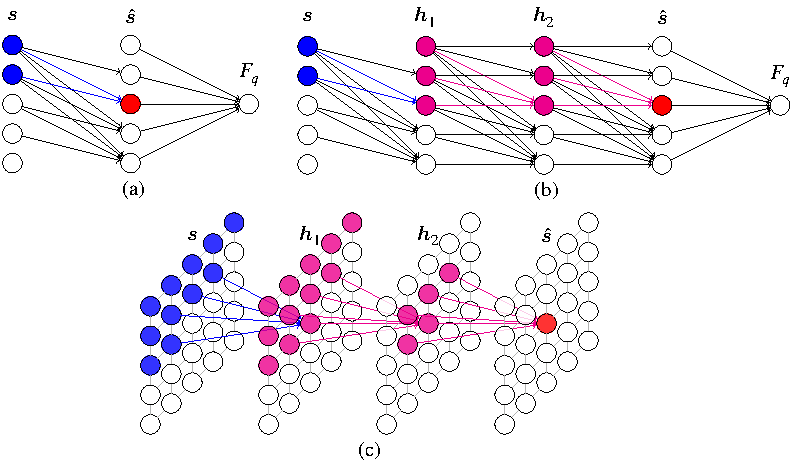
\includegraphics[width=0.9\linewidth]{ch5/arnn_arch.pdf}
\caption[Architectures of autoregressive neural networks (ARNNs)]{
Architectures of dense and convolutional ARNNs for variational inference.
The spins $\vs$ are the inputs to the network.
The values $\hat{\vs}$ are the outputs from the network, which become parameters of the Bernoulli distributions.
The values $\vh_i$ are intermediate results in the network.
The variational free energy $F_q$ is given by \cref{eq:fq}, which depends on both the spins $\vs$ and the parameters $\hat{\vs}$.
The colored sites denote the receptive field of a site in $\hat{\vs}$, i.e., the input and the intermediate sites that an output site depends on.
(a) The network has only one layer, which is densely connected, and masked to ensure the AR property. The connections that are not masked out are illustrated as the arrows.
(b) The network has three masked dense layers.
(c) The network has three masked convolutional layers on a 2D lattice. In each layer, only the connections to one output site are shown for clarity, which depict the shape of the convolution kernel.
This figure is reproduced from Fig.~1 in Ref.~\cite{wu2019solving}.
}
\label{fig:arnn-arch}
\end{figure}

The most general way to parameterize the conditional probabilities is a dense feedforward neural network (FFNN) as in \cref{eq:ffnn}, which takes the spins $\vs$ as inputs, and outputs the parameters $\hat{\vs}$, then the conditional probabilities are modeled by the Bernoulli distributions $\calB(s_i \mid \hat{s}_i)$. The network needs to fulfill the AR property: each output $\hat{s}_i$ can only depend on the previous inputs $\vs_{< i}$. For a single dense layer, this is achieved by applying a triangular mask on the weight matrix in \cref{eq:linear-layer}:
\begin{gather}
\text{MaskedLin}(\vx) = (\mM \odot \mW) \vx + \vb, \\
M_{i j} = \begin{cases}
1, & i > j \\
0, & i \le j
\end{cases},
\end{gather}
where $\odot$ denotes the element-wise multiplication. This masked linear layer is illustrated in \cref{fig:arnn-arch}~(a). Multiple linear layers can be applied to improve the expressiveness of the network, and only one layer needs to mask out the connections $M_{i i}$, as shown in \cref{fig:arnn-arch}~(b). This architecture is known as the masked autoencoder for distribution estimation (MADE)~\cite{germain2015made}.

Convolutional layers can also be applied to utilize the translational symmetry and the locality of the physical system, with the same mask $\mM$ to ensure the AR property. However, unlike a single convolutional FFNN, the joint probability $q(\vs)$ of a convolutional ARNN is not translational invariant as in \cref{eq:trans-invar}. The ARNN always assigns an artificial order of the spins to factorize the joint probability, thus breaks the translational symmetry. Instead, the purpose of convolutions in ARNN should be understood as enforcing the translational invariance of certain rules to determine the effect of the local environment on a spin.

An early application of 1D convolutional ARNN is the modeling of audios, known as WaveNet~\cite{oord2016wavenet}. The 2D convolutional ARNN has been similarly applied to the modeling of images, known as PixelCNN~\cite{oord2016pixel}, whose shape of the 2D convolutional kernel is illustrated in \cref{fig:arnn-arch}~(c). These ARNN architectures have also been introduced to the modeling of many-body systems, originally under the name of variational autoregressive networks (VANs)~\cite{wu2019solving}, and achieved superior results compared to traditional variational ansatzes.

Besides the dense and the convolutional ones, another widely used family of ARNNs are the recurrent neural networks (RNNs), which incorporate the translational symmetry of the physical system in another way. They maintain the AR property by updating of some hidden variables $\vh^{(i)}$, also known as ``memories'', at each AR step $i$:
\begin{align}
\vh^{(i)} &= f\left( s_{i - 1}, \vh^{(i - 1)} \right), \label{eq:rnn-update} \\
\hat{s}_i &= g\left( \vh^{(i)} \right), \label{eq:rnn-output}
\end{align}
where $f$ and $g$ can be arbitrarily sophisticated neural networks, and their parameters are usually shared between sites. Because of the parameter sharing, RNNs can achieve satisfactory results with fewer parameters than dense networks. More variants of RNNs, including hybrids with CNNs and tensor networks, are also used in practice~\cite{oord2016pixel, khandoker2023supplementing}. Notably, the popular large language models in modern machine learning have essentially inherited the principles of RNN~\cite{brown2020language}. It is also worth mentioning that ARNNs with hierarchical architectures~\cite{bialas2022hierarchical} and representations in frequency and wavelet spaces~\cite{nash2021generating, mattar2024wavelets} have been proposed to enhance the translational symmetry and the scalability.

\subsection{Numerical results}

\begin{figure}[htb]
\centering
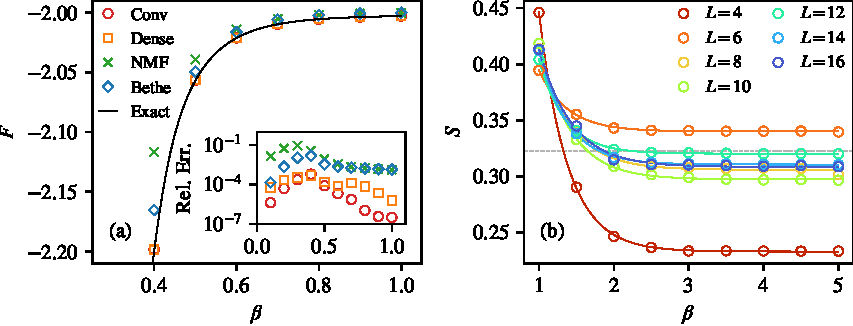
\includegraphics[width=\linewidth]{ch5/arnn_ising.pdf}
\caption[ARNN results of Ising model on square and triangular lattices]{
(a) Free energy per site $F / N$ of the ferromagnetic (FM) Ising model on the $16 \times 16$ square lattice with periodic boundary conditions (PBC), at varying inverse temperature $\beta$, given by a dense ARNN and a convolutional ARNN, compared to the exact result~\cite{onsager1944crystal} and the traditional methods of naive mean-field (NMF) and Bethe ansatzes.
The inset shows the relative error of the numerical results compared to the exact result. \\
(b) Entropy per site $S / N$ of the frustrated antiferromagnetic (AFM) Ising model on triangular lattices of different sizes $N = L \times L$ with PBC, given by a convolutional ARNN.
The curves are least-square fittings of $S / N = a \rme^{-b \beta} + c$, where $a, b, c$ are parameters for fitting, and $c$ is the residual  entropy when $\beta \to \infty$.
The horizontal dashed line indicates the exact result $\lim_{N \to \infty} \lim_{\beta \to \infty} S / N \approx 0.323$~\cite{wannier1950antiferromagnetism, wannier1973antiferromagnetism}.
Note that the curves for $L = 8, 14, 16$ are almost overlapped.
This figure is reproduced from Fig.~2 in Ref.~\cite{wu2019solving}.
}
\label{fig:arnn-ising}
\end{figure}

\subsubsection{Square Ising model}

We first demonstrate the performance of ARNN on the well-studied ferromagnetic (FM) Ising model on the $10 \times 10$ square lattice with periodic boundary conditions (PBC), where the analytical result~\cite{onsager1944crystal} and the traditional methods of naive mean-field (NMF) ansatz in \cref{sec:nmf} and Bethe ansatz in \cref{sec:bethe} are available for comparison. A dense ARNN and a convolutional ARNN are trained on the Boltzmann distribution of this Hamiltonian, whose hyperparameters, such as the number of layers, the number of channels, and the convolution kernel size are selected to produce the lowest variational free energies within a reasonable computation budget. The networks are trained from scratch at each inverse temperature $\beta = 0.1, 0.2, \ldots, 1$. \Cref{fig:arnn-ising}~(a) shows the results of free energy, where we can clearly see that the ARNNs produce superior results compared to the traditional ansatzes, whose relative errors are lower by orders of magnitude.

In particular, the results from the convolutional ARNN are generally more accurate than those from the dense one with a similar number of parameters, thanks to the utilization of the translational symmetry and the locality of the physical system. This comparison justifies the use of convolutional layers in ARNN, even though the overall joint probability is not translational invariant. However, this advantage diminishes around the critical point $\beta_c = \frac{1}{2} \ln(1 + \sqrt{2}) \approx 0.44$, where the correlation length of the physical system diverges until bounded by the system size, as discussed in \cref{sec:iat}. The convolutional neural network can capture these long-range correlations only if the size of its receptive field is at least comparable to the correlation length.

\subsubsection{Triangular Ising model}
\label{sec:arnn-tri-ising}

Then we apply the convolutional ARNN to the more complicated problem of antiferromagnetic (AFM) Ising model on the triangular lattice with PBC, which is geometrically frustrated. As discussed in \cref{sec:frustrate}, the frustration leads to exponentially many degenerate ground states and a non-zero residual entropy, which poses challenge for MCMC and previous variational ansatzes. In \cref{fig:arnn-ising}~(b), the ARNN produces entropies that exponentially decay to a constant as $\beta \to \infty$ for each system size $L$, and converge around the analytical result as $L \to \infty$. These results demonstrate the rich expressiveness of ARNN, which has the potential to accurately approximate exponentially complex target distributions using polynomial computation time and number of parameters.

\subsubsection{Hopfield model}
\label{sec:arnn-hop}

\begin{figure}[htb]
\centering
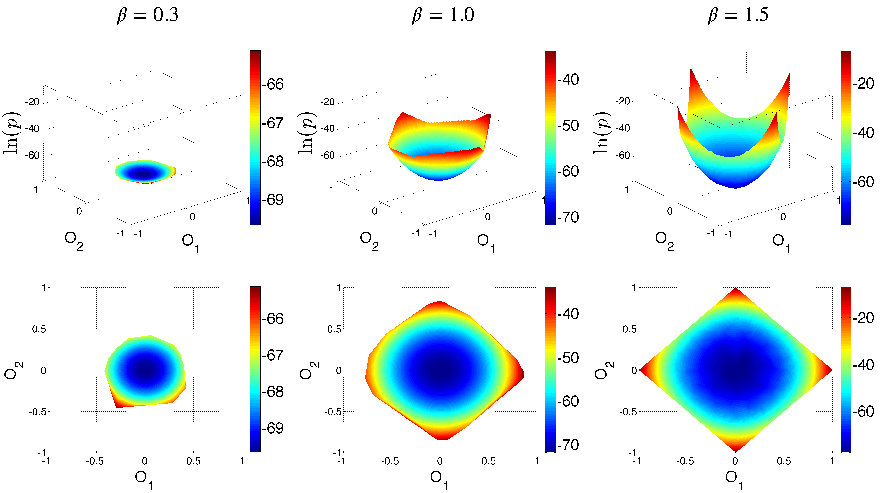
\includegraphics[width=\linewidth]{ch5/arnn_hop.pdf}
\caption[ARNN results of Hopfield model]{
Log-probability $\ln q$ of samples from a dense ARNN, for the Hopfield model with $N = 100$ spins and $n_\text{pat} = 2$ orthogonal patterns.
The top row shows the 3D view of the log-probability surfaces, and the bottom row shows the same results in the 2D view from top.
The columns are results with different inverse temperatures $\beta = 0.3, 1.0, 1.5$.
The $O_1$ and $O_2$ axes denote the overlaps between each sample and the two patterns respectively, as defined in \cref{eq:cl-overlap}.
The four ground states have $(O_1, O_2)$ = $(+1, 0)$, $(-1, 0)$, $(0, +1)$, $(0, -1)$ respectively.
This figure is reproduced from Fig.~3 in Ref.~\cite{wu2019solving}.
}
\label{fig:arnn-hop}
\end{figure}

An experiment to qualitatively study the ability of ARNN to capture multiple ground states is on the Hopfield model in \cref{sec:hopfield}. We construct a Hopfield model with $N = 100$ spins and $n_\text{pat} = 2$ random orthogonal patterns, and train a dense ARNN that only consists of a single layer. Then we generate $10^4$ samples from the ARNN, and compute their probabilities and their overlaps with the two patterns respectively. \Cref{fig:arnn-hop} shows that the ARNN successfully samples the memorized patterns with exponentially higher probabilities than other states, in the retrieval phase with high $\beta$. This indicates the capability of ARNN to avoid mode collapse and capture all the modes separated by exponentially high energy barriers in this Hamiltonian.

\subsubsection{Sherrington--Kirkpatrick (SK) model}

\begin{figure}[htb]
\centering
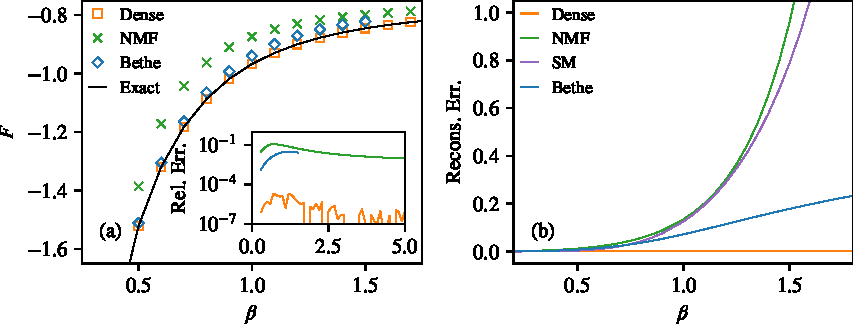
\includegraphics[width=\linewidth]{ch5/arnn_sk.pdf}
\caption[ARNN results of Sherrington--Kirkpatrick (SK) model and inverse SK problem]{
(a) Free energy per site $F / N$ for a random instance of the SK model with $N = 20$ spins, at varying inverse temperature $\beta$, given by a dense ARNN, compared to the exact result by enumeration, the NMF ansatz, and the Bethe ansatz. The inset shows the relative error of the numerical results compared to the exact result.
The iterative solution of the Bethe ansatz converges only when $\beta \le 1.5$. \\
(b) Reconstruction error of the inverse SK problem with $N = 20$ spins, given by a dense ARNN, compared to the NMF ansatz~\cite{roudi2009ising}, the Sessak--Monasson (SM) expansion~\cite{sessak2009small}, and the Bethe ansatz~\cite{ricci2012bethe}.
This figure is reproduced from Fig.~4 in Ref.~\cite{wu2019solving}.
}
\label{fig:arnn-sk}
\end{figure}

We also have the experiment on the Sherrington--Kirkpatrick (SK) model in \cref{sec:sk}, which has frustrated interactions with even higher complexity than the previous models. As a proof of concept, we generate a random instance of the SK model with $N = 20$ spins, and compute its properties by exact enumeration. Then we train a dense ARNN with a single layer. \Cref{fig:arnn-sk}~(a) shows that the ARNN still produces substantially more accurate approximation than traditional ansatzes for this Hamiltonian, especially in the glassy phase with high $\beta$ where the iterative solution of the Bethe ansatz fails to converge.

\subsubsection{Inverse SK problem}

Besides the ordinary problem of estimating the observables given the Hamiltonian, ARNNs can also be employed in the inverse SK problem, where we estimate the unknown interactions $\{J^*_{i j}\}$ given the correlations $\{C^*_{i j}\}$. Because each estimated correlation $\bbE_\text{MC}[C_{i j}]$ as in \cref{eq:monte-carlo} is a differentiable function of $\{J_{i j}\}$, we can directly use stochastic gradient descent to minimize the least-square loss
\begin{equation}
L\left( \{J_{i j}\} \right) = \frac{1}{N^2} \sum_{i j} \left( \bbE_\text{MC}[C_{i j}] - C^*_{i j} \right)^2.
\end{equation}
In this problem, we use an ARNN with two dense layers to estimate $C_{i j}$. The abilities of different methods to estimate the interactions is assessed by the reconstruction error
\begin{equation}
\text{Recons. Err.} = \frac{1}{N^2} \sum_{i j} \left( J_{i j} - J^*_{i j} \right)^2,
\end{equation}
where $J_{i j}$ are the estimated values and $J^*_{i j}$ are the true values. The results are shown in \cref{fig:arnn-ising}~(b), where the ARNN again outperforms traditional methods by a large margin.

\subsection{Remarks on network sizes and computation times}

It is worth discussing the sizes of the ARNNs used in the above experiments. For the fully connected cases of the Hopfield model, the SK model, and the inverse SK problem, we use small ARNNs containing only $O(N^2)$ parameters which take minutes to train on a high-end GPU as of this writing, and they produce substantially better results than the Bethe ansatzes with the same order of parameters. For the Ising models on the $16 \times 16$ square and triangular lattices, however, the ARNNs with the optimal variational free energies we have found contain as many as $O(10^6)$ parameters, while the Bethe ansatzes only contain $O(10^3)$. The large number of parameters also leads to substantially more computation time to evaluate the observables, as the training and the sampling of such a large neural network typically take hours on a high-end GPU, while the NMF ansatz and the Bethe ansatz can be solved almost instantly. Therefore, many use cases of neural networks to replace traditional ansatzes appear only in the regime where we seek for much higher accuracy at the cost of correspondingly more computation. The comparison of neural networks and traditional methods under the same computation budget will be discussed in \cref{sec:arnn-mcmc}.

Apart from training a new network with each system size and temperature, it has also been proposed to directly reuse or fine-tune a trained network with different system sizes and temperatures~\cite{efthymiou2019super, mills2019extensive, rende2024fine}. This line of research opens a promising way to numerically compute the renormalization group (RG) flow, and extrapolate the critical temperature to the thermodynamic limit~\cite{ron2002inverse}.

\section{Sparse two-body ARNN (TwoBo)}
\label{sec:twobo}

In the previous section, we have seen that the simple ARNN with dense architecture approximates many-body systems to much higher accuracy than traditional ansatzes, but also introduces much more trainable parameters and requires longer computation time. The convolutional ARNN reaches even higher accuracy with the same amount of parameters, as it utilizes the translational symmetry and the locality of the physical system. In this section, we continue to seek for a more sophisticated ARNN architecture that further embodies knowledge of the physical system, particularly the sparsity, to reduce the number of trainable parameters and the computation time without losing the expressiveness.

An approach has been proposed in Ref.~\cite{pan2021solving} to convert any many-body system on a sparse graph into an equivalent system on a smaller dense graph using the feedback vertex set. Meanwhile, it has been noticed in Ref.~\cite{pr2021analysis} that the dense ARNN architecture involves a lot of redundant computation that can be eliminated given the physical properties of the Boltzmann distribution and the locally interacting Hamiltonian. In the following, we present a different approach proposed in Ref.~\cite{biazzo2024sparse}, which utilizes these physical properties to improve the efficiency of ARNN.

\subsection{TwoBo architecture from Boltzmann distribution}

We start from directly factorizing the many-body Boltzmann distribution $p_\text{B}(\vs)$ into AR conditional distributions in \cref{eq:autoreg}:
\begin{equation}
p_{\text{B} i}(s_i \mid \vs_{< i})
= \frac{\sum_{\vs_{> i}} p_\text{B}(\vs)}{\sum_{\vs_{\ge i}} p_\text{B}(\vs)}
= \frac{\sum_{\vs_{> i}} \rme^{-\beta H(\vs)}}{\sum_{\vs_{\ge i}} \rme^{-\beta H(\vs)}},
\end{equation}
and simplifying the result. When the Hamiltonian has only two-body interactions, such as the Ising model in \cref{eq:cl-ising-general}, it has been derived in Ref.~\cite{biazzo2024sparse} that the conditional probability takes the form:
\begin{align}
p_{\text{B} i}(s_i = +1 \mid \vs_{<i}) &= S\left( 2 \beta \xi_{i i} + \rho_{\text{B} i}\left( \{\xi_{i l} \mid l > i\} \right) \right), \label{eq:twobo} \\
\xi_{i l} &= \sum_{k < i} J_{k l} s_k, \label{eq:twobo-xi}
\end{align}
in the notations of this thesis, and omitting the external fields for simplicity. Here $S$ is the sigmoid function in \cref{eq:sigmoid}, and $\rho_{\text{B} i}$ is a function depending on $\mJ$ and $\beta$. The function $\rho_{\text{B} i}$ is different for each index $i$, and it only takes the intermediate variables $\xi_{i l}$ with $l > i$ as the inputs. Although the exact evaluation of $\rho_{\text{B} i}$ can take exponential time, it has been shown in Ref.~\cite{biazzo2023autoregressive} that $\rho_{\text{B} i}$ can be simplified for specific physical systems, such as an analytical expression for the Curie--Weiss model and a replica symmetric breaking (RSB) approximation for the SK model.

\begin{figure}[htb]
\centering
\hspace*{\fill}
\subfloat[]{\raisebox{0.055\linewidth}{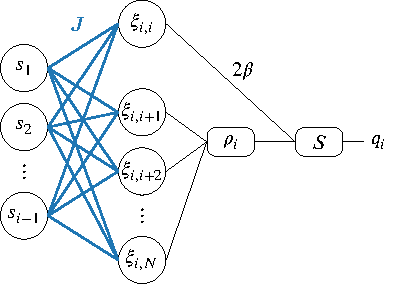
\includegraphics[width=0.4\linewidth]{ch5/twobo_arch.pdf}}}
\hspace*{\fill}
\subfloat[]{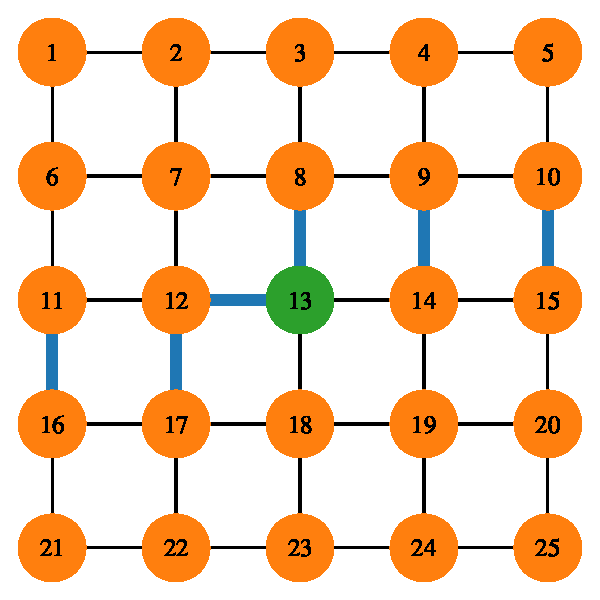
\includegraphics[width=0.4\linewidth]{ch5/twobo_grid_2d.pdf}}
\hspace*{\fill}
\caption[Architecture of the sparse two-body ARNN (TwoBo)]{
(a) Sketch of the TwoBo ARNN architecture to compute a conditional probability $q_i(s_i = +1 \mid \vs_{< i})$.
The weights of the first layer are directly taken from the interaction matrix $\mJ$ and fixed.
The function $\rho_i$ is parameterized by a dense layer, whose inputs are the variables $\{\xi_{i l} \mid l > i\}$ after the first layer.
The last activation function $S$ is the sigmoid function in \cref{eq:sigmoid}, and there is a skip connection from $\xi_{i i }$ to $S$ with the fixed weight $2 \beta$. \\
(b) Calculating the conditional probability $q_i(s_i \mid \vs_{< i})$ with $i = 13$ on a 2D grid of $N = 25$ spins. The edges between the spins $\vs_{< i}$ and $\vs_{\ge i}$ are highlighted in blue, and only these edges are used when computing the intermediate variable $\xi_{i l}$. Therefore, among the variables $\{\xi_{i l} \mid l > i\}$, only those with $l < i + L$ are kept as inputs to $\rho_i$, and the others are ensured to be zero, which enhances the sparsity of the TwoBo network.
This figure is reproduced from Fig.~1 in Ref.~\cite{biazzo2024sparse}.
}
\label{fig:twobo-arch-grid}
\end{figure}

For the purpose of this thesis, we approximate $\rho_{\text{B} i}$ using a neural network $\rho_i$ with trainable parameters, and we have surprisingly found that using a single dense layer is enough to obtain results with satisfactory accuracies in our numerical experiments. Also, we interpret the linear transformation from the input spins $s_i$ to the intermediate variables $\xi_{i l}$ in \cref{eq:twobo-xi} as another linear layer without bias, whose weights are directly taken from $\mJ$ and not trained. Therefore, \cref{eq:twobo} becomes an ARNN ansatz $q_i(s_i \mid \vs_{< i})$ as shown in \cref{fig:twobo-arch-grid}~(a). This architecture is colloquially named TwoBo, because the authors were tired of the ever-growing lengths of acronyms.

\subsection{Sparsity of intermediate variables}
\label{sec:twobo-sparse}

The incorporation of the interaction matrix $\mJ$ into the parameters of TwoBo leads to the opportunity of reducing the computation time and the number of trainable parameters using the sparsity of the physical system. In general, the first layer in \cref{eq:twobo-xi} can be evaluated by a matrix-vector multiplication $\mJ \vs$ while storing cumulative sums, which takes $O(N^2)$ time, where $N$ is the number of spins. When the physical system is sparse and the number of non-zero entries in $\mJ$ only scales by $O(N)$, the evaluation takes only $O(N)$ time as well.

For each function $\rho_i$, there are $N - i$ input variables in general and a scalar output, which introduces $O(N)$ parameters and $O(N)$ computation time when parameterized by a single dense layer. Fortunately, when the physical system has a local geometry, many of the input variables are ensured to be zero. For example, on a 2D grid with $N = L^2$ spins as shown in \cref{fig:twobo-arch-grid}~(b), each variable $\xi_{i l}$ is non-zero only when $i < l < i + L$, thus the number of input variables to $\rho_i$, the number of parameters in it, and the time to evaluate it are all reduced from $O(L^2)$ to $O(L)$. Considering all the functions $\{\rho_i \mid 1 \le i \le N\}$, they take $O(L N) = O(L^3)$ time to evaluate in total, which dominates over the $O(N)$ time of the first layer. Those functions also have $O(L^3)$ parameters in total. Therefore, the time to evaluate the TwoBo ansatz and the number of trainable parameters in it both scale by $O(L^3)$, which is polynomially lower than $O(L^4)$ of the dense ARNN (MADE) in \cref{sec:made}. Similarly, the time and the space are reduced from $O(L^6)$ to $O(L^5)$ on 3D grids.

\subsection{Numerical results}
\label{sec:twobo-results}

The performance of TwoBo is demonstrated in numerical experiments using the Edwards--Anderson (EA) model with binary interactions on 2D and 3D grids with PBC, as well as random regular graphs (RRGs). As discussed in \cref{sec:ea}, the EA model is generally more difficult to solve than the simple Ising model in \cref{sec:made}, and the 3D EA model is particularly challenging from the perspective of computational complexity. Moreover, the RRG demonstrates the performance of TwoBo on systems without regular geometry. We use RRGs with degree $d = 3$, and sample them from the uniform distribution of all RRGs with the given $N$ and $d$ using the Steger--Wormald algorithm~\cite{steger1999generating}. Each reported result is averaged over $10$ random instances of the Hamiltonian, and the error bar shows the standard error over the instances.

The results from TwoBo are compared with those from MADE. We use the MADE with only one layer, and it still has more trainable parameters than the TwoBo with the same system size. On the 2D grids, another comparison is made with the RNN architecture in Ref.~\cite{hibat2021variational}, which has outperformed several dense and convolutional ARNN architectures in the regime of numerous parameters. In this thesis, we mainly compare with it in the regime of few parameters, using only four memory units and a comparable number of trainable parameters to TwoBo, while the comparison using more parameters will be shown in \cref{fig:twobo-rnn-param}.

An annealing procedure is performed to compute the free energies at different inverse temperatures $\beta \in (0, 3]$, and help the optimization converge to the desired global minimum at high $\beta$. We equally divide the range of $\beta$ into $N_\text{anneal} = 60$ annealing steps. At the first $\beta = 0.05$, we perform $N_\text{warm} = 500$ optimization steps as warm-up. After that, in each annealing step, we perform $N_\text{opt} = 200$ optimization steps while keeping $\beta$ unchanged. In the next annealing step, we continue to optimize the ansatz with a different value of $\beta$. All the architectures of TwoBo, MADE, and RNN are trained using this procedure.

\subsubsection{Variational free energy and ground state energy}

\begin{figure}[htb]
\centering
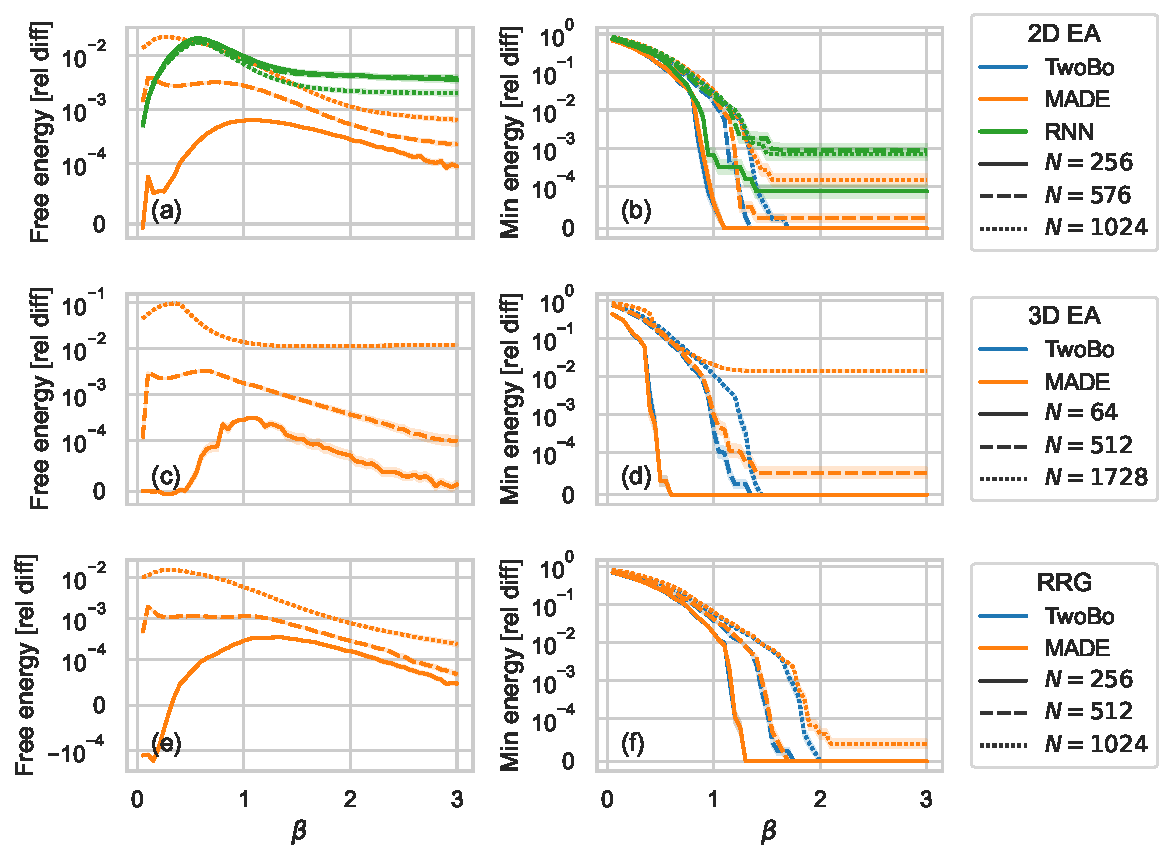
\includegraphics[width=\linewidth]{ch5/twobo_ea.pdf}
\caption[TwoBo results of Edwards--Anderson (EA) model]{
Variational free energy (left column) and minimum energy of sampled configurations (right column) at varying inverse temperature $\beta$, for the EA model on 2D grids (top row), 3D grids (middle row), and RRGs (bottom row) of different sizes.
The performances of TwoBo, MADE, and RNN (only in 2D) architectures are compared.
The variational free energy is shown as the relative difference from TwoBo at the same $\beta$, and the minimum energy is relative from the one found by TwoBo at $\beta = 3$.
The $y$-axis uses the logarithmic scale when the absolute value is greater than $10^{-4}$.
This figure is reproduced from Fig.~2 in Ref.~\cite{biazzo2024sparse}.
}
\label{fig:twobo-ea}
\end{figure}

As shown in the left column of \cref{fig:twobo-ea}, TwoBo gives lower variational free energy than MADE and RNN with comparable numbers of trainable parameters, on almost all tested geometries, system sizes, and temperatures, except in the simple cases of low $\beta$. This demonstrates the accuracy of TwoBo in approximating the Boltzmann distribution, even with disordered and frustrated Hamiltonians, and this advantage becomes more substantial at larger system sizes.

The right column of \cref{fig:twobo-ea} shows the minimum energy found by the ansatzes in the annealing procedure, which is of more interest in combinatorial optimization problems. TwoBo is also able to find lower energies than MADE and RNN, especially at large system sizes. In addition to variational methods, we also use the exact solvers in McGroundstate~\cite{charfreitag2022mcsparse} and the heuristic solvers in MQLib~\cite{dunning2018what} to solve the same systems. Compared to these solvers, TwoBo gives equal or lower energies with comparable computation time in all tested cases, which provides evidence that the sophisticated heuristics of neural networks outperform traditional methods in optimization problems with many variables and complicated interactions.

\subsubsection{Convergence of training}

\begin{figure}[htb]
\centering
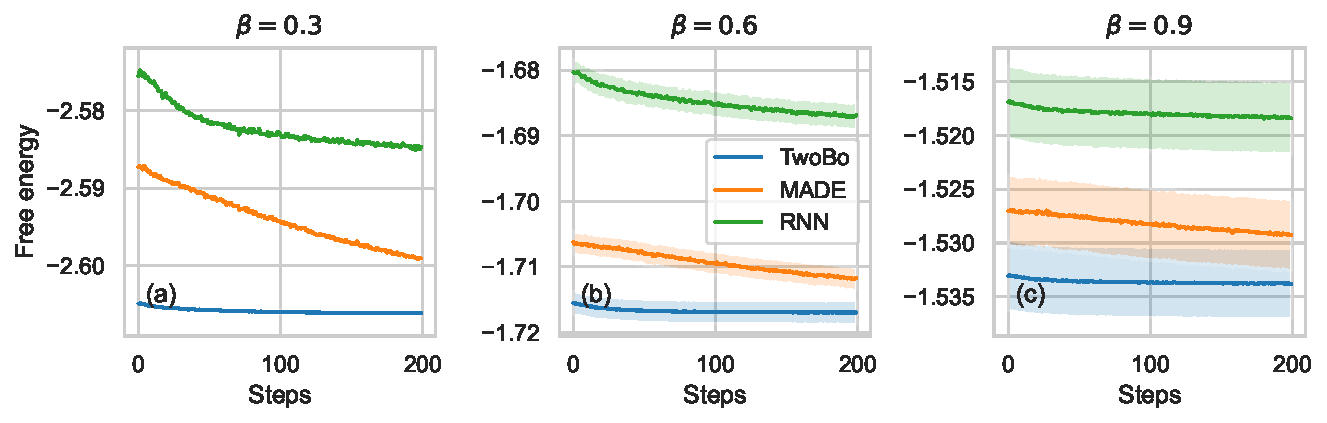
\includegraphics[width=\linewidth]{ch5/twobo_converge.pdf}
\caption[Convergence of TwoBo variational free energy in training]{
Convergence of variational free energy during the optimization steps in an annealing step, at different inverse temperatures $\beta$, on the 2D EA model with $N = 576$.
This figure is reproduced from Fig.~3 in Ref.~\cite{biazzo2024sparse}.
}
\label{fig:twobo-converge}
\end{figure}

\begin{figure}[htb]
\centering
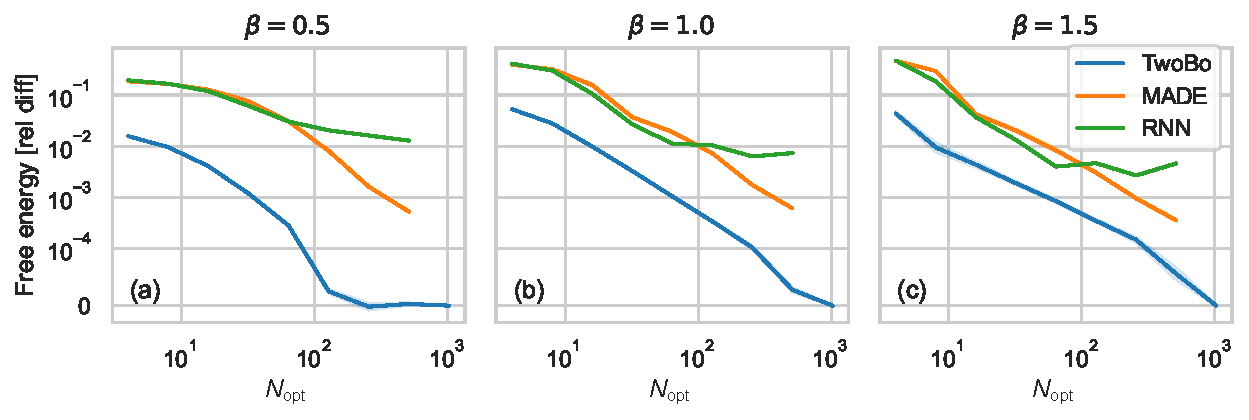
\includegraphics[width=\linewidth]{ch5/twobo_n_opt.pdf}
\caption[TwoBo variational free energy vs.\ annealing speed]{
Variational free energy as a function of the annealing speed, at different inverse temperatures $\beta$, on the 2D EA model with $N = 576$.
The annealing speed is controlled by the number of optimization steps $N_\text{opt} = 4, 8, 16, \ldots, 1024$ in each annealing step.
The variational free energy is shown as the relative difference from TwoBo at the same $\beta$ with $N_\text{opt} = 1024$.
The $y$-axis uses the logarithmic scale when the value is greater than $10^{-4}$.
This figure is reproduced from Fig.~4 in Ref.~\cite{biazzo2024sparse}.
}
\label{fig:twobo-n-opt}
\end{figure}

Besides the accuracy after training, TwoBo also has the advantage of fast convergence during training. As shown in \cref{fig:twobo-converge}, in each annealing step with a fixed $\beta$, TwoBo always starts from a lower variational energy, and reaches convergence in fewer optimization steps. This advantage can be attributed to the incorporation of the interactions $\mJ$ in the parameters, which makes the initialization of the ansatz $q(\vs)$ physically feasible, i.e., closer to the target distribution $p_\text{B}(\vs)$ than a neural network with only random initialization.

This fast convergence also allows us to reduce the total computation time of the annealing procedure using a higher annealing speed. The annealing speed is controlled by the number of optimization steps $N_\text{opt}$ in each annealing step. As shown in \cref{fig:twobo-n-opt}, the variational free energy systematically decreases as $N_\text{opt}$ increases, presumably in a power law. In particular, TwoBo reaches the same variational free energy with almost an order of magnitude smaller $N_\text{opt}$ than MADE and RNN, which demonstrates its high efficiency in training. Therefore, we use only $N_\text{opt} = 200$ to achieve satisfactory results in \cref{fig:twobo-ea}, and each training can finish in an hour on a high-end GPU.

\subsubsection{Parameter efficiency}

\begin{figure}[htb]
\centering
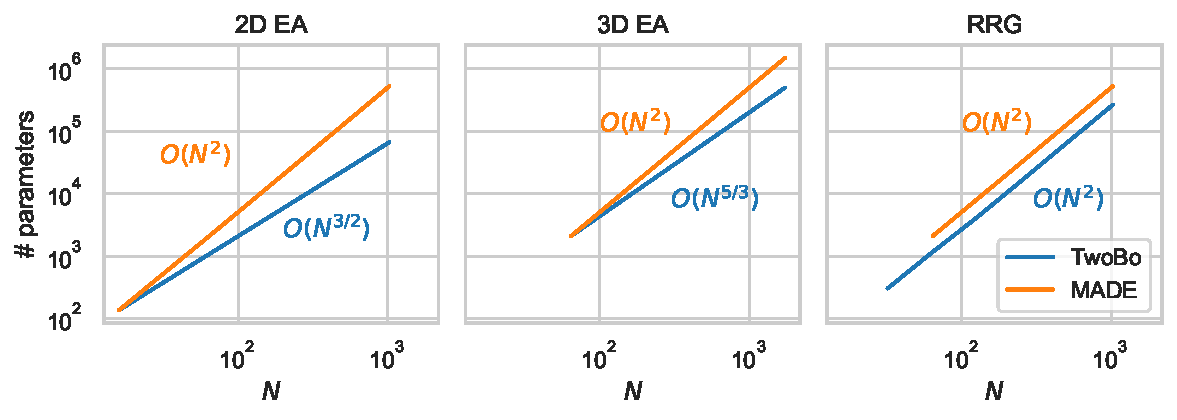
\includegraphics[width=\linewidth]{ch5/twobo_param.pdf}
\caption[Number of parameters vs.\ system size for TwoBo and MADE]{
Number of trainable parameters in TwoBo and MADE as a function of the system size $N$, on 2D grids, 3D grids, and RRGs.
This figure is reproduced from Fig.~S1 in the supplementary material for Ref.~\cite{biazzo2024sparse}.
}
\label{fig:twobo-param}
\end{figure}

\begin{figure}[htb]
\centering
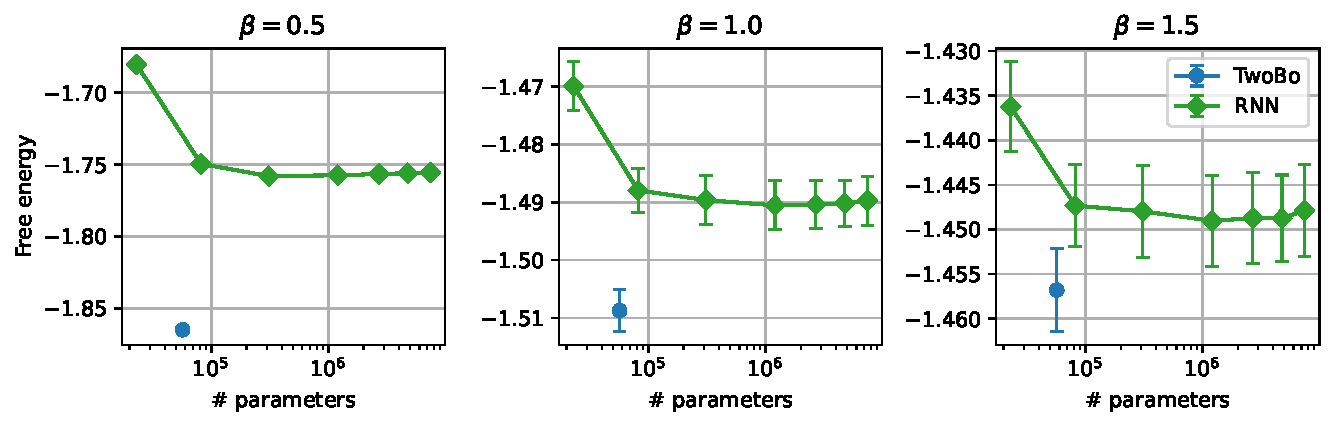
\includegraphics[width=\linewidth]{ch5/twobo_rnn_param.pdf}
\caption[Variational free energy vs.\ number of parameters for TwoBo and RNN]{
Variational free energy of TwoBo compared to RNN with different numbers of memory units ($2, 4, 8, 16, 24, 32, 40$), on the 2D EA model with $N = 576$.
This figure is reproduced from Fig.~S3 in the supplementary material for Ref.~\cite{biazzo2024sparse}.
}
\label{fig:twobo-rnn-param}
\end{figure}

Lastly, we investigate the empirical scaling of the number of trainable parameters in TwoBo with the system size. As shown in \cref{fig:twobo-param}, TwoBo has polynomially fewer parameters than MADE on 2D and 3D grids. For the RRGs without a local geometry, however, TwoBo no longer has polynomially fewer parameters, but only fewer by a constant coefficient of approximately $2$. These results are consistent with the theoretical analysis in \cref{sec:twobo-sparse}.

This advantage is more sharply demonstrated when we compare with RNN in the regime of numerous parameters. As shown in \cref{fig:twobo-rnn-param}, the TwoBo with few parameters gives lower variational free energy than the RNN with a comparable number of parameters, and even if we enlarge the RNN by orders of magnitude, the variational free energy does not systematically decrease. These results emphasize the importance of the lightweight architecture with the physical knowledge in TwoBo, which can be more efficient than scaling up a general neural network architecture with increasing computation.

\subsection{Conclusion}

In conclusion, the TwoBo architecture incorporates the knowledge of the Boltzmann distribution and the sparse two-body interacting Hamiltonian into the neural network design, therefore achieves more accurate free energy estimation, faster training speed, and polynomially higher parameter efficiency compared to previous ARNN architectures. It opens a promising way to scale up the variational inference computation to larger systems, and extract more physically interpretable results from neural networks.

\section{ARNN in importance sampling}
\label{sec:arnn-mcmc}

In the previous sections, we have seen the advantages of ARNN over previous ansatzes in variational inference. Meanwhile, as discussed in \cref{sec:compare-mcmc}, when unbiased estimations of observables rather than an upper bound of the free energy is desired, we can also use ARNN with the importance sampling in \cref{eq:importance-sampling} and the MCMC importance sampling in \cref{eq:mcmc-importance}.

Soon after Ref.~\cite{wu2019solving} introduced ARNN in statistical physics problems, Ref.~\cite{nicoli2020asymptotically} has proposed to use ARNN in the importance sampling and the MCMC importance sampling. However, Ref.~\cite{ciarella2023machine} has questioned the efficiency of these sampling methods on physical systems with complicated probability landscapes, such as the Potts model and the random graph coloring problem in the random first-order transition (RFOT) universality class. Moreover, Ref.~\cite{bialas2023analysis} has noticed that a reliable analysis of the autocorrelation time in \cref{eq:iat} is largely overlooked in the studies of these sampling methods, which is crucial for measuring the efficiency of MCMC methods. Fortunately, as discussed in \cref{sec:mode-collapse}, cluster update methods and symmetry operations can help overcome the problem of mode collapse in first-order phase transitions, while reducing the autocorrelation time as well.

In the following, we present a sampling method proposed in Ref.~\cite{wu2021unbiased}, which constructs cluster updates using the AR property of the ansatz, and applies the symmetries of the physical system, to achieve the unbiased sampling with high efficiency even if the physical system exhibits a first-order phase transition.

\subsection{Neural cluster updates with symmetries (NCUS)}
\label{sec:ncus}

\begin{algorithm}[H]
\caption[Neural cluster updates with symmetries (NCUS)]{
A sampling step in NCUS for a system of $N$ spins on a square lattice with translation, $D_4$ lattice reflection, and $\bbZ_2$ spin flipping symmetries.
}
\label{alg:ncus}
\begin{algorithmic}[1]
\STATE Input the current configuration $\vs$
\STATE Sample an integer $k \in \{1, \ldots, N\}$ from the distribution $P_\text{cluster}(k)$
\STATE Sample the last $k$ spins and propose the configuration $\vs'$
\STATE Accept $\vs \gets \vs'$ with the probability in \cref{eq:ncus-a}
\STATE Translate $\vs$ by a random displacement
\STATE Reflect $\vs$ along the $x$-axis, the $y$-axis, and the diagonal, each with $50\%$ probability
\STATE Reflect $\vs$ along the $z$-axis (flip all spins) with $50\%$ probability
\STATE Output $\vs$ as a sample in the Markov chain
\end{algorithmic}
\end{algorithm}

\begin{figure}[htb]
\centering
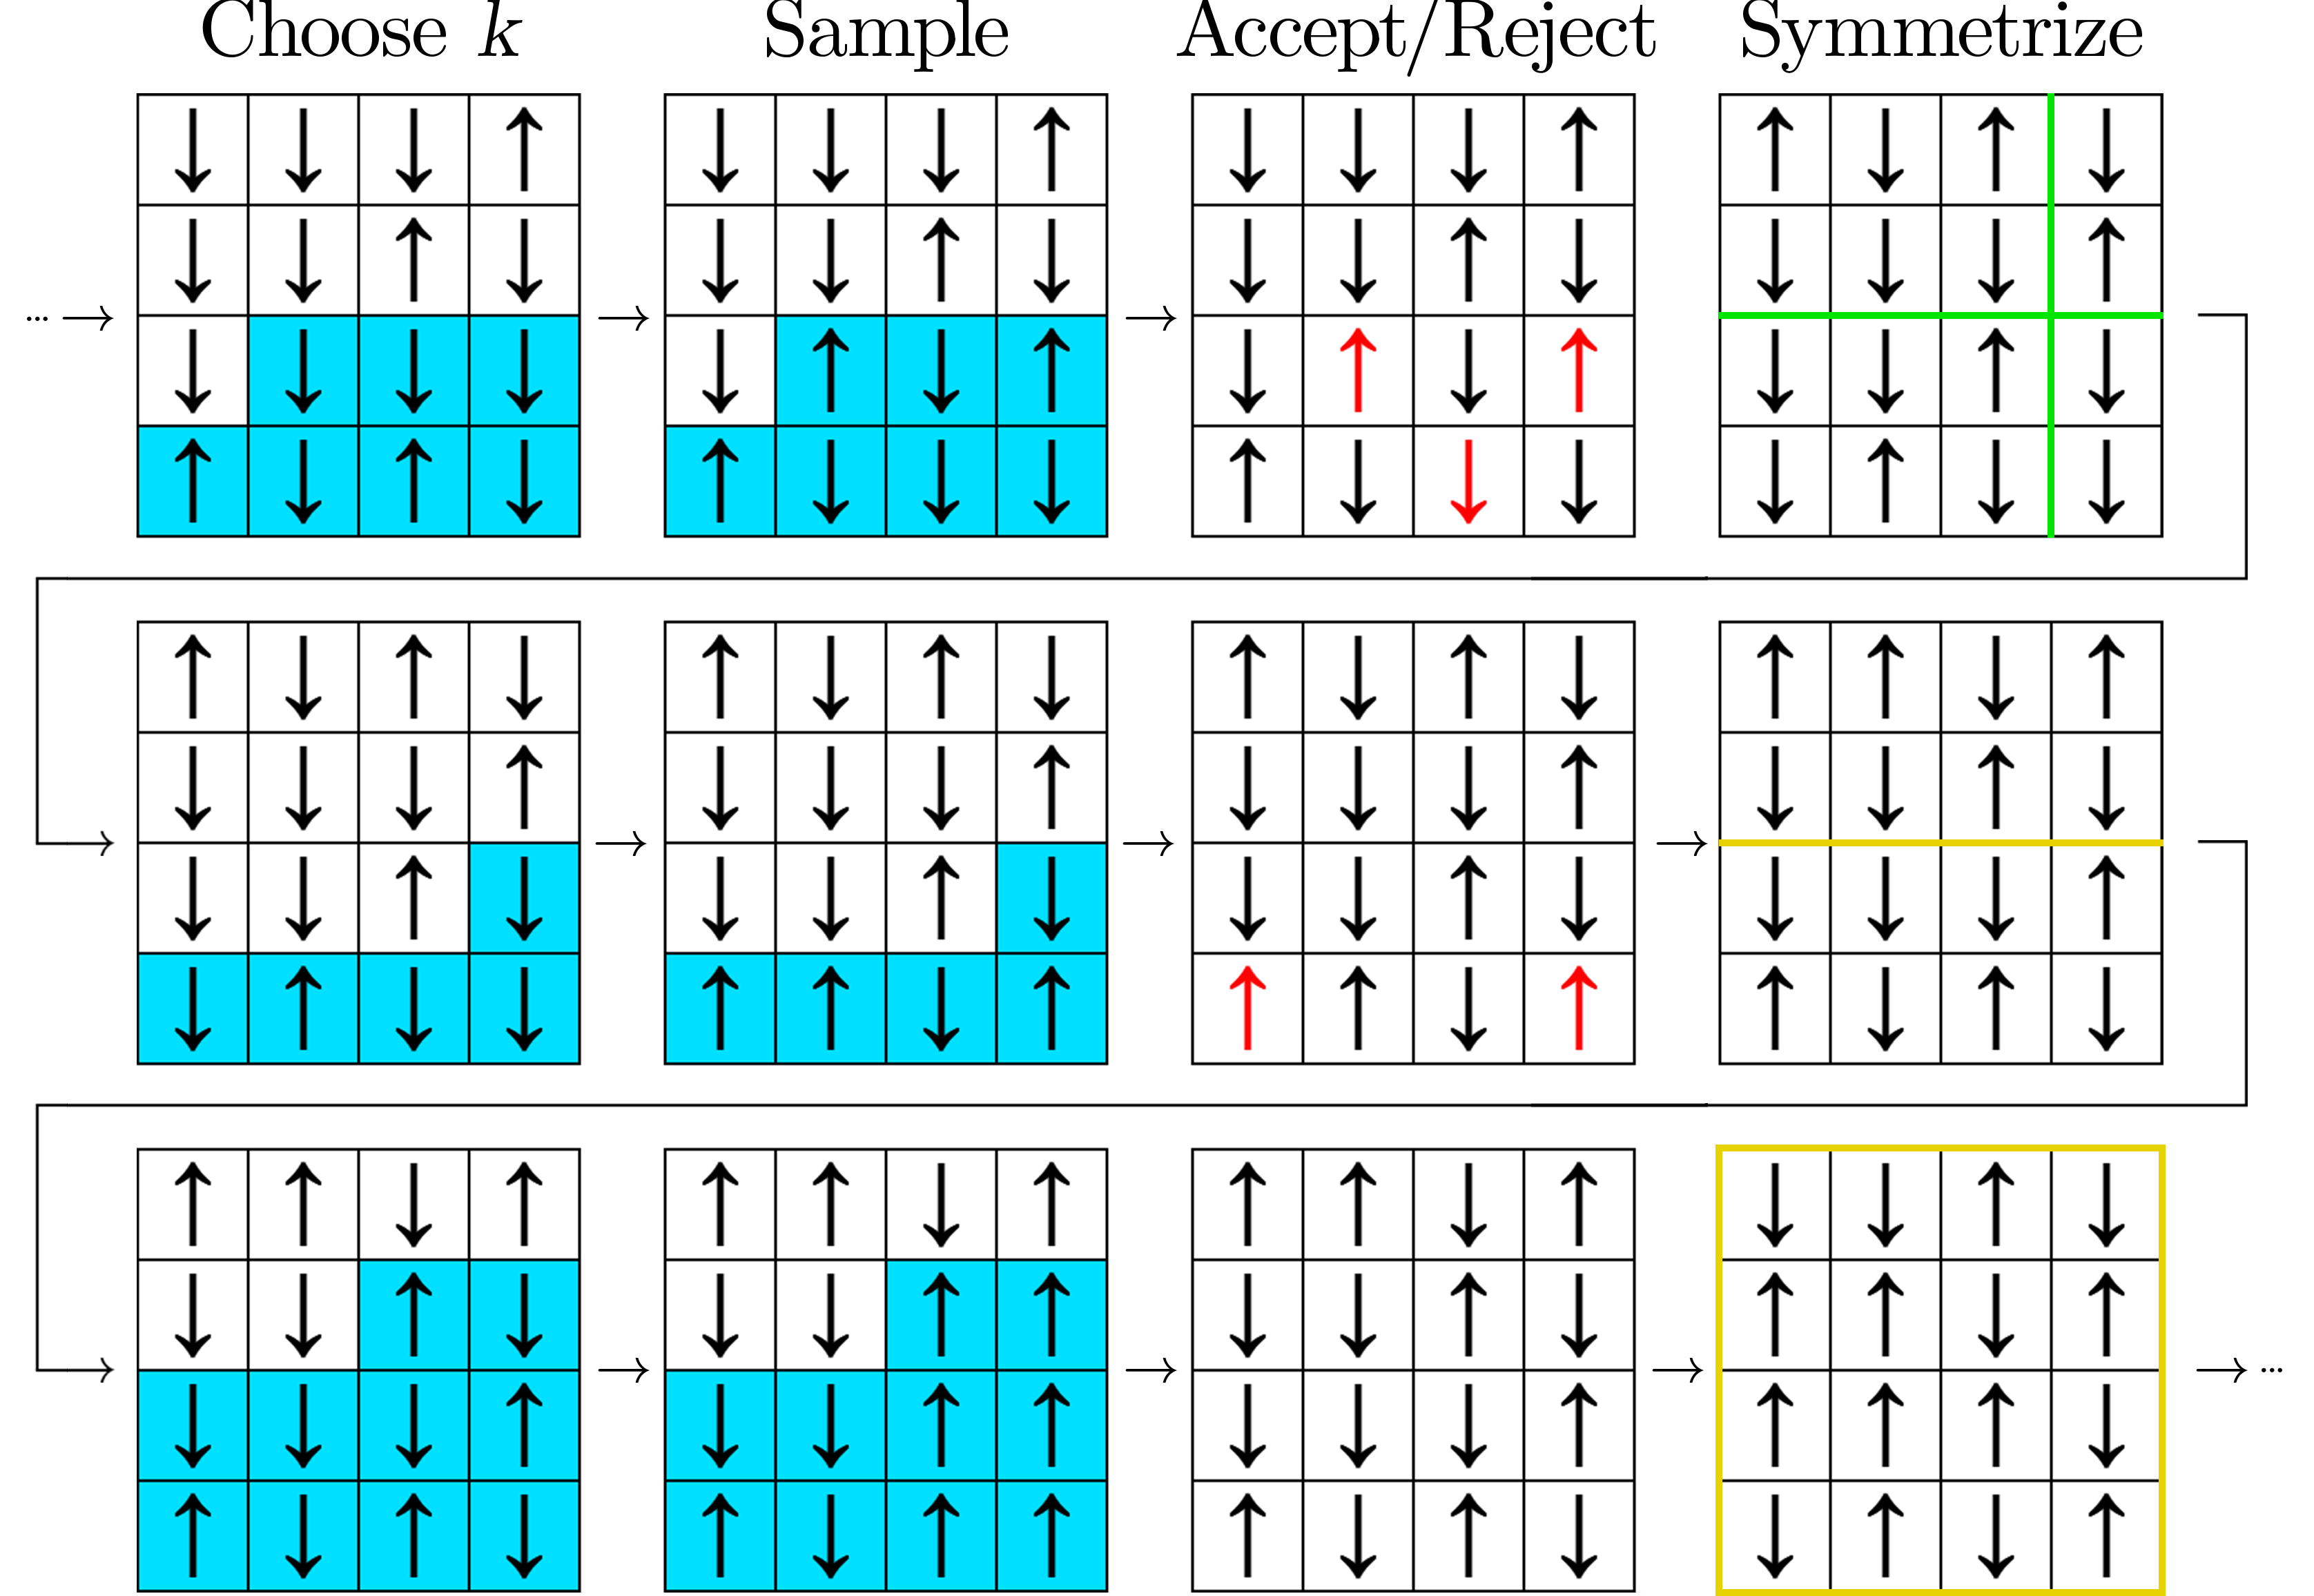
\includegraphics[width=0.6\linewidth]{ch5/ncus_proc.png}
\caption[Procedure of neural cluster updates with symmetries (NCUS)]{
Examples of three steps of NCUS applied to a system on the $4 \times 4$ square lattice. The operations in several lines of \cref{alg:ncus} are visualized by colors.
In line $2$, the last $k$ spins chosen are highlighted in {\color[HTML]{1f77b4} blue}.
In line $3$, some of them are flipped in the proposal.
Then in line $4$, if the proposal is actually accepted, the flipped spins are shown in {\color[HTML]{d62728} red}.
In line $5$, the original borders of the lattice before the translation are shown in {\color[HTML]{2ca02c} green}.
In line $6$, the plane of reflection is shown in {\color[HTML]{bcbd22} yellow}, and a reflection along the $z$-axis (across the $x y$-plane) is indicated by yellow borders around the lattice.
This figure is reproduced from Fig.~1 in Ref.~\cite{wu2021unbiased}.
}
\label{fig:ncus-proc}
\end{figure}

During the MCMC importance sampling procedure in \cref{eq:mcmc-importance}, we propose new configurations $\vs'$ from the ansatz $q(\vs)$. When the ansatz is factorized into the AR conditional distributions in \cref{eq:autoreg}, we can notice that it is possible not to generate all the $N$ spins from the beginning, but only the last $k$ spins. In this way, the acceptance in \cref{eq:mcmc-importance} becomes
\begin{equation}
A(\vs \to \vs') = \min\left( 1, \frac{p(\vs')}{p(\vs)} \prod_{i = N - k + 1}^N \frac{q_i(s_i \mid \vs_{< i})}{q_i(s'_i \mid \vs'_{< i})} \right),
\label{eq:ncus-a}
\end{equation}
which is usually close to $1$ when $k$ is small. With suitable values of $k$, we can enjoy the efficiency of cluster updates, which overcome both the inability of local updates to transition through energy barriers and the low acceptance probability of global updates. We refer to the distribution of $k$ as $P_\text{cluster}(k)$, and it can be the uniform distribution over $\{1, \ldots, N\}$ without loss of generality. Comparisons between choices of $P_\text{cluster}(k)$ will be presented in \cref{fig:ncus-pk}.

The construction of the above clusters introduces an obvious bias that the spins closer to the end of the autoregressive order will be more frequently flipped. To flip every spin with the same frequency on average, we randomly apply the symmetry operations of the Hamiltonian to the samples in the Markov chain. These operations act as global updates that transition through local energy barriers, and they are never rejected because they conserve the energy and thus have an acceptance probability of $1$. Combining the cluster updates and the symmetry operations, we refer to the resulting algorithm as neural cluster updates with symmetries (NCUS). This algorithm is described in \cref{alg:ncus} and visualized in \cref{fig:ncus-proc}.

\subsection{Numerical results}

\subsubsection{Ising model}

\begin{figure}[htb]
\centering
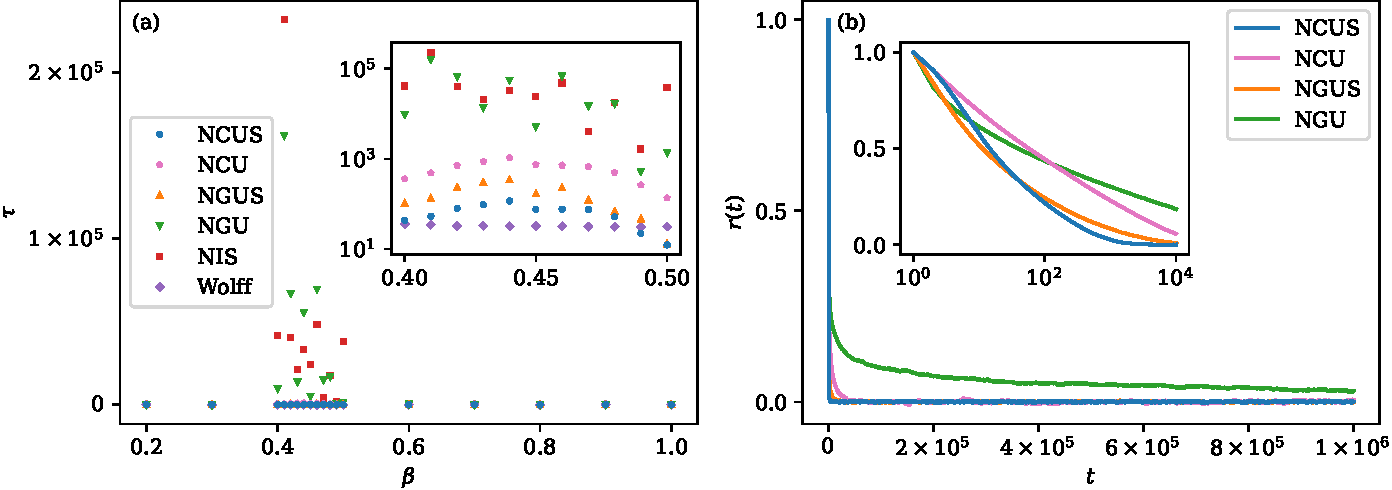
\includegraphics[width=\linewidth]{ch5/ncus_ising_autocorr.pdf}
\caption[NCUS results of Ising model]{
(a) Autocorrelation time $\tau$ for the Ising model on the $16 \times 16$ square lattice, at varying inverse temperature $\beta$, given by the sampling methods in this section.
The inset focuses on their behaviors around the critical point and uses the logarithmic scale on the $y$-axis. \\
(b) Normalized autocorrelation $r(t)$ at $\beta = 0.44$ around the critical point.
The inset uses the logarithmic scale on the $x$-axis to focus on their behaviors at small $t$.
This figure is reproduced from Fig.~2 in Ref.~\cite{wu2021unbiased}.
}
\label{fig:ncus-ising-autocorr}
\end{figure}

To demonstrate the performance of NCUS, we first conduct numerical experiments using the Ising model on the square lattice with PBC, which has translation, $D_4$ lattice reflection, and $\bbZ_2$ spin flipping symmetries. We compare NCUS with \cref{eq:importance-sampling}, referred to neural importance sampling (NIS) here, as well as \cref{eq:mcmc-importance}, referred to as neural global updates (NGU) here. As ablation studies, we also consider neural global updates with symmetries (NGUS) and neural cluster updates (NCU) without symmetries. In addition, the well-established Wolff cluster update algorithm~\cite{wolff1989collective} is taken for comparison.

In all the neural sampling methods, we use a same neural network trained using the usual variational method. The network is a convolutional ARNN with approximately $4 \times 10^3$ parameters, which is much smaller compared to the networks used in \cref{sec:made}, as we now emphasize the efficient sampling and the correction to the non-ideally trained ansatz $q(\vs)$. After the sampling, the mean free energies given by all the methods are apparently close to each other, so we focus on analyzing the autocorrelation times of the free energy as defined in \cref{eq:iat}, which determine the error bars. For NIS, although it does not produce a Markov chain, we use the effective sample size in \cref{eq:eff-sample-size,eq:eff-sample-size-w} to define an effective autocorrelation time for comparison.

As shown in \cref{fig:ncus-ising-autocorr}~(a), around the critical point, NCUS produces autocorrelation times lower by orders of magnitude than the previous neural sampling methods, while the autocorrelation times from NGU and NIS are pathologically high. A closer look at the normalized autocorrelation functions in \cref{fig:ncus-ising-autocorr}~(b) confirms these results, where the samples from NCUS quickly decorrelate in less than $10^3$ steps, while those from NGU cannot decorrelate after as many as $10^5$ steps. Moreover, the autocorrelation times from NCUS is comparable to those from the Wolff algorithm, even though the latter is specifically designed for the Ising model. These results illustrate the advantage of cluster updates and symmetry operations in alleviating the problem of critical slowing down, as discussed in \cref{sec:critical-slow}.

\subsubsection{Frustrated plaquette model (FPM)}
\label{sec:ncus-fpm}

\begin{figure}[htb]
\centering
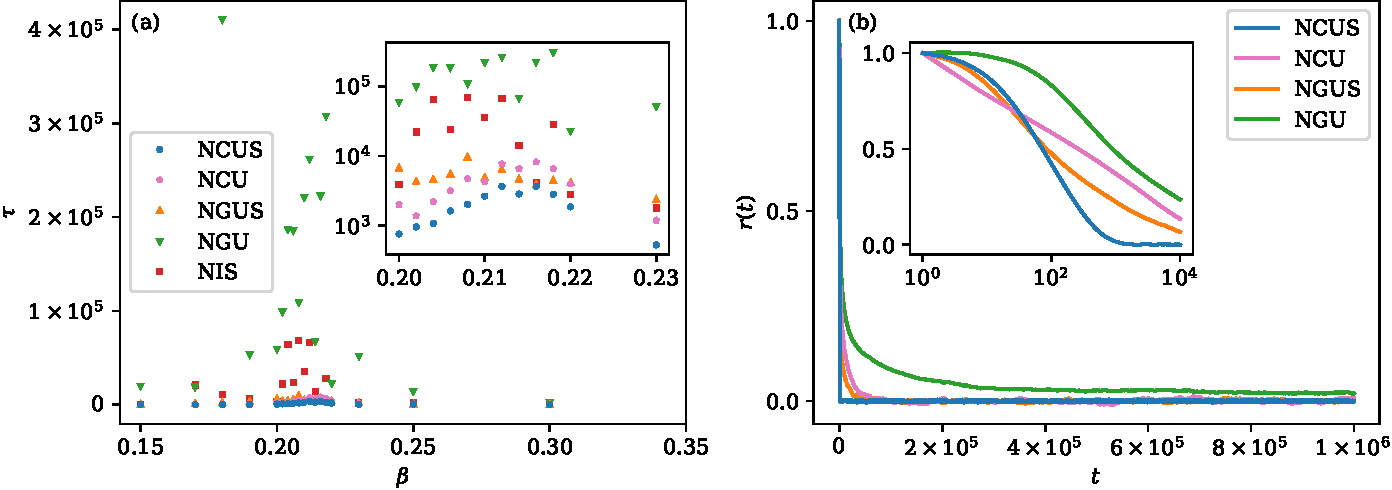
\includegraphics[width=\linewidth]{ch5/ncus_fpm_autocorr.pdf}
\caption[NCUS results of FPM]{
(a) Autocorrelation time $\tau$ for the FPM on the $32 \times 32$ square lattice, at varying inverse temperature $\beta$, given by the sampling methods in this section.
The inset focuses on their behaviors around the critical point and uses the logarithmic scale on the $y$-axis. \\
(b) Normalized autocorrelation $r(t)$ at $\beta = 0.2$ around the critical point.
The inset uses the logarithmic scale on the $x$-axis to focus on their behaviors at small $t$.
This figure is reproduced from Fig.~4 in Ref.~\cite{wu2021unbiased}.
}
\label{fig:ncus-fpm-autocorr}
\end{figure}

Next, we apply the sampling methods to the frustrated plaquette model (FPM) discussed in \cref{sec:fpm}, which is more difficult than the Ising model due to the first-order phase transition induced by the frustrated $J_3$ interactions and the plaquette interactions. Moreover, we increase the system size from $16 \times 16$ to $32 \times 32$. This time, the Wolff algorithm is no longer applicable as it is designed only for systems with two-body interactions. In contrast, the neural sampling methods are general enough to handle the plaquette interactions.

As shown in \cref{fig:ncus-fpm-autocorr}, the results have a similar trend to those for the Ising model around the critical point. The autocorrelation times from NCUS can be as high as $O(10^3)$, but it is still practical to obtain reliable estimations of the free energy with the error bars derived from them, and they are lower by orders of magnitude than the results from the previous neural sampling methods. These results provide evidence that cluster updates and symmetry operations help alleviate the problem of mode collapse with the presence of first-order phase transitions aforementioned in \cref{sec:mode-collapse}.

\subsubsection{Choices of the distribution $P_\text{cluster}(k)$}

\begin{figure}[htb]
\centering
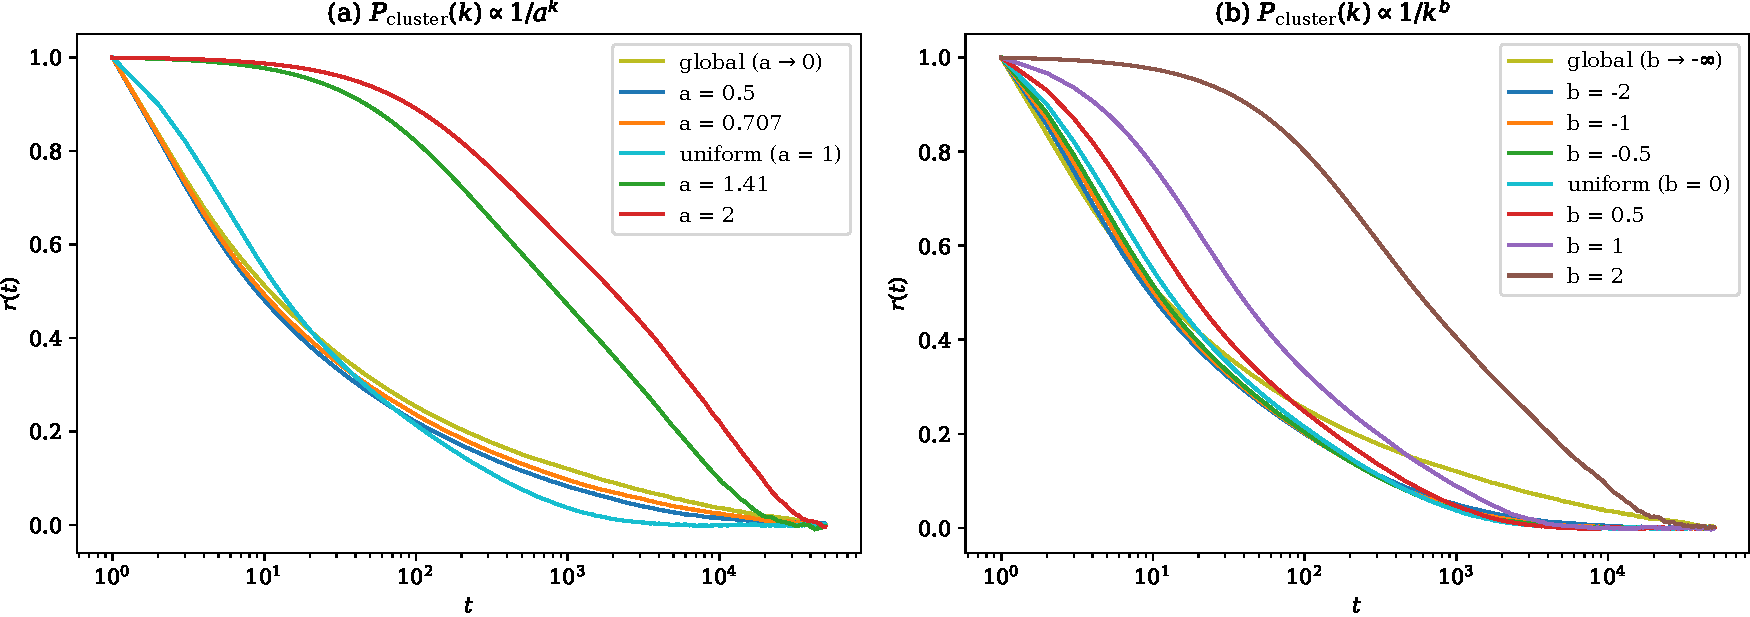
\includegraphics[width=\linewidth]{ch5/ncus_pk.pdf}
\caption[Choices of the distribution $P_\text{cluster}(k)$ in NCUS]{
Normalized autocorrelation $r(t)$ given by NCUS on the $16 \times 16$ Ising model at inverse temperature $\beta = 0.44$, with different choices of $P_\text{cluster}(k)$ from exponential and power distributions.
This figure is reproduced from Fig.~S1 in the supplemental material for Ref.~\cite{wu2021unbiased}.
}
\label{fig:ncus-pk}
\end{figure}

The efficiency of NCUS can depend on the distribution $P_\text{cluster}(k)$ of the number of spins to generate. In the above results, we have arbitrarily chosen the uniform distribution. The empirical comparisons between different choices of exponential distributions $P_\text{cluster}(k) \propto 1 / a^k$ and power distributions $P_\text{cluster}(k) \propto 1 / k^b$, where $a$ and $b$ are adjustable parameters, are shown in \cref{fig:ncus-pk} respectively. The uniform distribution gives comparable or lower autocorrelation time than all other distributions we have tested. Moreover, it also outperforms the more naive method of always using the same number, i.e., $P_\text{cluster}(k) = \delta(k - k')$ for all $k' \in \{1, \ldots, N\}$. It remains an open question to reveal the relation between the optimal $P_\text{cluster}(k)$ and the properties of the target distribution $p(\vs)$ as well as the ansatz $q(\vs)$, using theoretical analysis on the Markov chain transitions.

\subsection{Conclusion}

In conclusion, the NCUS algorithm utilizes the cluster updates constructed by the AR property of the ansatz, as well as the symmetries of the physical system, to produce substantially lower autocorrelation times than the conventional global update method around the critical point, and more reliable estimations of observables with lower error bars in consequence.

We look forward to more research combining the strengths of the techniques presented in this section, including the neural networks as highly expressive heuristics for complicated multivariate distributions, autoregressive models with exact sampling and normalized probability evaluation, physical properties such as symmetries and sparsity incorporated into network architectures, and cluster updates that alleviate the problems of critical slowing down and mode collapse, which will eventually lead to solutions for physical systems with unprecedented size and complexity.
